\documentclass[sigconf,nonacm]{acmart}
\settopmatter{printacmref=false,printccs=false,printfolios=true}
\setcopyright{none}
\acmDOI{}\acmISBN{}\acmConference{}{}{}
\acmYear{2026}\copyrightyear{2026}
\usepackage{graphicx,booktabs,array,balance}
\graphicspath{{figures/}}
\begin{document}
\emergencystretch=1em
\title{Shrinking Code: Reuse, Reliability, and Cost in Ten Car-Yard Skills}
\author{Omar Dylan Abou}\email{odabou@ncsu.edu}
\affiliation{\institution{North Carolina State University}\city{Raleigh}\state{NC}\country{USA}}
\author{Henoc Dossou}\email{hbdossou@ncsu.edu}
\affiliation{\institution{North Carolina State University}\city{Raleigh}\state{NC}\country{USA}}
\author{Andrew Sergison}\email{arsergis@ncsu.edu}
\affiliation{\institution{North Carolina State University}\city{Raleigh}\state{NC}\country{USA}}
\renewcommand{\shortauthors}{Abou, Dossou, and Sergison}
\begin{abstract}
We test incremental reuse in ten car-yard skills across six Claude-generated conditions and nine complete V2 repetitions. Of 540 planned outcomes, 440 pass, 32 fail syntax, eight fail competency, and 60 are blocked. Six matched, fully generated standalone/reuse pairs show 37.2--48.8\% less final source with reuse; five pairs also satisfy all competency and regression checks. Reuse does not consistently improve reliability, and its estimated cost is often higher. Separate AI-assisted coursework and native-EZR adapters pass all ten checks once each. We report interrupted runs, conditional quality, and the limits of our comparisons.
\end{abstract}
\keywords{software reuse, generated code, empirical software engineering}
\maketitle
\noindent\textbf{Repository:} \url{https://github.com/OmarDylan/shrinking-code-project}
\section{Hypotheses}
\textbf{The Timm hypothesis.} Neuro-symbolic systems improve when their symbolic half is factored into small reusable structures. The ten skills are synonyms: one machine (cluster, tree, leaf) wearing ten hats. Hence an LLM, or a human, extends a well-factored library with less new code, and fewer errors, than a monolithic one.

\textbf{The rival.} The ten skills are ten separate problems. Factoring buys nothing: skill i+1 costs about the same whoever writes it, and whatever library sits underneath.\cite{course}

Our client is a used-car dealership. Auto93 contains 398 cars (318 training, 80 held out), with weight, acceleration and economy objectives. Falling new-code shares, successful delivery, and fewer errors would favor the Timm hypothesis; flat shares or no consistent improvement favor the rival. We separately measure final LOC, cost and task quality.
\section{Requirements}
The client wish list in \texttt{docs/requirements.md} maps two asks to each skill. Table~\ref{tab:req} condenses all twenty without changing their intent.
\begin{table}[h]
\caption{Customer asks (numbered and skill-tagged).}\label{tab:req}\centering\scriptsize
\begin{tabular}{@{}lp{.77\columnwidth}@{}}\toprule
Skill & Customer asks\\\midrule
Remember & (1) Find great buys; (2) show typical good, average and poor cars.\\
Guess & (3) Estimate fuel use before the sticker; (4) judge a listing from partial specs.\\
Certify & (5) Decide whether one group really beats another; (6) tell if a recommendation gain matters.\\
Flow & (7) Judge cars as they arrive; (8) warn when incoming quality changes.\\
Blame & (9) Explain why poor cars are slow, heavy or thirsty; (10) identify specs associated with bad buys.\\
Justify & (11) Explain why one car wins; (12) explain acceptance/rejection to a skeptical buyer.\\
Choose & (13) Find a great car with few test drives; (14) find alternatives without inspecting everything.\\
Fix & (15) Suggest the smallest improvement; (16) show changes making a car resemble better cars.\\
Spot & (17) Flag odd listings that may be erroneous or scams; (18) find unusual cars even if not poor.\\
Race & (19) Compare selection with random choice; (20) find good cars with fewer inspections.\\\bottomrule
\end{tabular}
\end{table}
\section{Methods}
\textbf{Controlled arms.} T1/T2 use plain Python, T3/T4 have scikit-learn available, T5/T6 have EZR source available. Odd arms generate separate skill files; even arms extend earlier source and rerun previous checks. Assigned-library availability does not require import. T7 is an AI-assisted adapter to earlier EG5/EG6 coursework, not the required unaided-human control. E1 is a separate post-hoc AI-assisted adapter invoking pinned native EZR functions; it is not another randomized arm.

\textbf{Reset and evaluation.} Each of R02--R05, R07--R10 and R12 is a fresh Claude Sonnet generation path under frozen V2 contracts: one-shot headless calls, fresh temporary directories, no retained conversations, and no repair of valid completed syntax failures. Train-only fitting and masked held-out goals are used where prescribed. R01 is a pilot; R06, R11 and R13 are interrupted and excluded from the complete-repetition set. R13 was an attempted replacement for R11; its timeout led to stopping at $N=9$, short of the ten-repeat rubric target. Session-limit/OAuth rejections with confirmed zero usage were archived and recovered; unknown-cost timeouts were not retried. We evaluate immutable snapshots in restricted containers; dependency versions match, image digests differ. We separate generated syntax failures, competency failures, and downstream blocking. A delivered run passes all ten individual checks and, for reuse, all ten regression-step checks.

\textbf{Measurement.} We retain physical LOC added/removed, final accumulated LOC, tokens, estimated API-equivalent generation cost and wall time. A repetition path is the unit, not cars or Race episodes. Course-style \texttt{same} requires pooled Cohen $\leq .35$, absolute Cliff $\leq .195$ and scaled KS $\leq 1.36$; this diagnostic is distinct from the fixed Certify threshold $.197$. Comparisons with fewer than three observations per group are labeled insufficient. Quality summaries condition on passing snapshots; no zero scores are imputed for failures.
\section{Results}
\begin{table}[t]
\caption{Nine repetitions per controlled arm: 90 planned outcomes each.}\label{tab:results}\centering\scriptsize
\begin{tabular}{@{}lrrrrrr@{}}\toprule
 & T1 & T2 & T3 & T4 & T5 & T6\\\midrule
Pass &84&48&79&68&79&82\\
Syntax &6&4&9&3&9&1\\
Competency fail &0&2&2&0&2&2\\
Blocked &0&36&0&19&0&5\\
Full delivery (/9)&4&4&1&6&1&7\\
Cost (USD)&2.70&4.10&2.55&5.18&6.39&11.93\\\bottomrule
\end{tabular}
\end{table}
Of 540 outcomes, 440 (81.5\%) pass; 32 fail syntax, eight fail competency and 60 are blocked (Table~\ref{tab:results}). All 448 valid generated snapshots are evaluated. T1 has the highest observed individual pass count, T6 the highest observed full-delivery count. These are descriptive, not universal rankings. In R12 T6, Blame strips the goal-name suffixes required by the contract; Justify consumes the same incorrect names. Both fail and subsequent regression checks retain the errors.
\begin{figure}[t]
\centering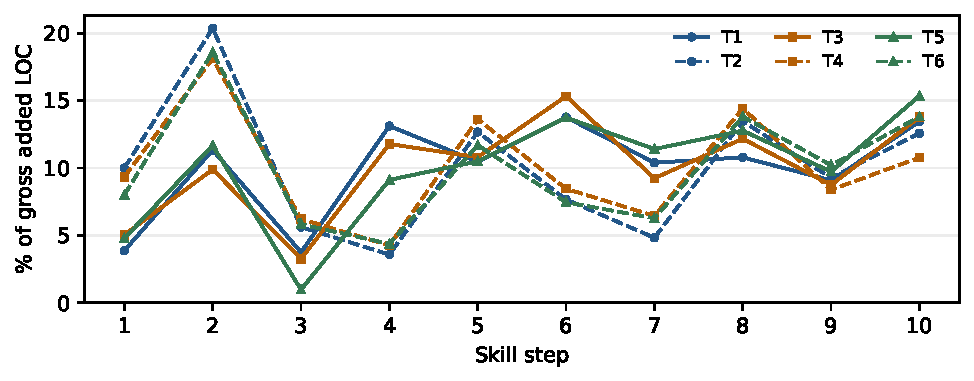
\includegraphics[width=\linewidth]{step_shares.pdf}
\Description{Six line series of measured gross added source code shares at steps one through ten.}
\caption{Gross added physical LOC share by skill step, aggregated across recorded generated snapshots; partial runs included. Missing/blocked snapshots have no measured LOC. Not a tag-derived history; no uniform falling ladder.}\label{fig:steps}
\end{figure}
\begin{table}[t]
\caption{Complete-generation matched pairs; one pair fails competency.}\label{tab:loc}\centering\scriptsize
\begin{tabular}{@{}llrrrl@{}}\toprule
Run & Pair & No reuse & Reuse & Less & Both deliver?\\\midrule
R02 &T1/T2&1003&618&38.4\%&Yes\\
R02 &T3/T4&872&522&40.1\%&Yes\\
R03 &T3/T4&918&509&44.6\%&No\\
R04 &T1/T2&988&597&39.6\%&Yes\\
R05 &T1/T2&990&622&37.2\%&Yes\\
R09 &T5/T6&978&501&48.8\%&Yes\\\bottomrule
\end{tabular}
\end{table}
\textbf{Code size.} All six matched complete-generation pairs save 37.2--48.8\% of final physical LOC with reuse (Table~\ref{tab:loc}). Only five pairs deliver all skills and regressions. Across all nine paths per pair, gross additions are lower in all 27 reuse-versus-no-reuse comparisons; blocked tasks make low gross LOC an ambiguous success measure. The complete pairs are selected on successful generation, and the step profiles in Figure~\ref{fig:steps} do not consistently decline. The complete-pair sample sizes (3, 2, 1) limit inference.
\begin{table}[t]
\caption{Course-style \texttt{same} diagnostics for nine paths per arm. C, D, K denote Cohen, absolute Cliff and scaled KS. All rows fail at least one threshold.}\label{tab:same}\centering\scriptsize
\begin{tabular}{@{}llrrrr@{}}\toprule
Metric & Pair & C & D & K & Same?\\\midrule
Gross LOC&T1/T2&2.60&1.00&2.12&No\\
&T3/T4&2.22&1.00&2.12&No\\
&T5/T6&3.55&1.00&2.12&No\\
Cost&T1/T2&.51&.11&1.18&No\\
&T3/T4&1.24&.56&1.65&No\\
&T5/T6&1.79&.85&1.89&No\\
Pass count&T1/T2&1.10&.30&.94&No\\
&T3/T4&.39&.30&1.18&No\\
&T5/T6&.22&.51&1.41&No\\\bottomrule
\end{tabular}
\end{table}
\textbf{Cost and statistical limits.} The nine complete repetitions cost an estimated \$32.86; known project costs through the final interruption are \$33.24 (excluding R01, R06, auxiliary development and two unknown-cost later timeouts). This is not a subscription bill. Reuse costs more in 5/9, 7/9, and 8/9 matched paths, respectively. Growing prompt context may explain the trade-off. The \texttt{same} results in Table~\ref{tab:same} are exploratory distribution diagnostics, not formal causal significance tests; complete-case selection and multiplicity limit conclusions. Paired exact sign diagnostics for cost give $p=1.000,.180,.039$, unadjusted. No broad ranking is warranted. Full pairwise and per-step diagnostics are in the analysis supplement.
\begin{table}[t]
\caption{Conditional quality, upper medians of passing runs; T7 and E1 are single observations.}\label{tab:quality}\centering\scriptsize
\begin{tabular}{@{}lrrrr@{}}\toprule
Arm & MPG MAE $\downarrow$ & Flow agr. & Spot F1 & Race $\downarrow$\\\midrule
T1&3.979&.459&1.000&.1223\\
T2&3.999&.885&.976&.1139\\
T3&3.323&.721&.952&.1130\\
T4&3.359&.852&.850&.1130\\
T5&3.981&.459&.976&.1223\\
T6&3.937&.836&.952&.1139\\
T7&4.275&.656&1.000&.1313\\
E1&3.991&.770&.722&.1664\\\bottomrule
\end{tabular}
\end{table}
\textbf{Behavior and client value.} Passing does not guarantee useful outputs (Table~\ref{tab:quality}). Remember has exact top-ten reference precision/recall conditional on passing. Guess hit rates within $\pm2$ MPG are 23.75, 22.5, 50, 48.75, 25, 25, and 50\% for T1--T7, respectively; signed predictions were not retained for Spearman. Our external supplement compares T1--T7 using 336 fixed-case distribution diagnostics and 714 individual-snapshot/T7 diagnostics, with matched case IDs; these are not independent development tests. T7 has insufficient independent repetitions. Certify T5 passes only 2/9 despite 100\% accuracy on each successful run. Flow has four positive observed-score reference alerts per 61 eligible arrivals: never alerting achieves 93.4\% agreement. E1 detects 3/4; T7 detects 0/4. Spot F1 measures synthetic anomalies, not actual fraud. Choose inspects ten of 80 cars, and Fix tests hypothetical changes, not feasible mechanical repairs. Race uses 20 shared-data episodes; E1's adaptive best10=.1664 versus random=.1556 is \texttt{same} under its checker, not evidence of superiority.

\textbf{Actual EZR use.} None of the 165 generated T5/T6 snapshots directly imports EZR. E1 uses native table, tree, leaf, and acquisition functions with an adapter for the V2 interface (including normalization coefficient 1.702 versus native 1.7). E1 adds 259 LOC to 387 existing EZR LOC; T7 adds 437 LOC to 1,500 earlier coursework LOC. Both pass ten checks; E1 reproduces on the team's Mac. No independent authorship replication or timed development is measured. Native oracle acquisition uses checker-supplied labels; no separate self-tuning experiment was performed.
\begin{table}[t]
\caption{Individual pass counts by skill; nine planned per automated arm. The two references each pass ten checks once.}\label{tab:skillpass}\centering\small
\begin{tabular}{@{}lrrrrrr@{}}\toprule
Skill &T1&T2&T3&T4&T5&T6\\\midrule
Remember&6&5&7&7&9&9\\
Guess&9&5&7&7&8&9\\
Certify&7&5&6&7&2&9\\
Flow&9&5&9&7&7&9\\
Blame&9&4&7&7&9&7\\
Justify&9&4&9&7&9&7\\
Choose&9&5&8&7&8&8\\
Fix&9&5&9&7&9&8\\
Spot&9&5&9&6&9&8\\
Race&8&5&8&6&9&8\\
\bottomrule
\end{tabular}
\end{table}
\textbf{Skill-specific evidence.} Table~\ref{tab:skillpass} shows how complete-system reliability can diverge from task-specific reliability. Remember's exact numerical contract and the deterministic Blame, Justify and Fix contracts check defined outputs, not whether a dealership's staff find them useful. Choose may pass while selecting different cars; we retain selected-set overlap and regret separately. Fix reaches a modeled mean improvement of .4147 in each arm's passing-run upper median. This is a common frozen five-neighbor counterfactual contract, not evidence that physical changes are possible.

\section{Discussion}
We find conditional support for the source-size part of the Timm hypothesis: complete pairs consistently use fewer lines. We do not establish a monotonically shrinking skill ladder or uniformly fewer errors. Dependency cascades matter: T2 blocks 36 outcomes, while T6 delivers seven of nine full systems yet propagates two R12 errors through later snapshots. Reuse may save final code at the expense of larger prompts, and shorter incomplete programs are not better systems. Course-style diagnostics mark gross LOC, cost and pass-count distributions as not-same within each pair, but do not alone demonstrate a causal ranking. The limited complete-pair sample and unsuccessful deliveries weaken stronger claims.

\textbf{Client recommendations.} A dealership should treat the results as decision-support prototypes. A low MPG error is useful for screening incomplete listings, but prediction uncertainty must remain visible. Flow deserves a precision/recall evaluation rather than alert agreement alone: across the nine passing T6 runs, 9 positive reference alerts are found, 27 missed and 88 false alerts raised. E1 finds three of four in its single run, with 13 false alerts; this is not a proven production detector. Spot should send atypical listings to human inspection, not automatically label them scams. Certify's strict numerical pass criterion is useful for reproducibility, but a result on one dataset does not establish economic benefit. 

\textbf{Cost, completeness and uncertainty.} In the paired comparison, reuse consumes more measured generation time in 5/9, 7/9 and 8/9 paths. Those counts include prematurely stopped reuse paths. Even though the complete builds show useful savings, their selective inclusion cannot tell us how much code a failed treatment would have required to finish. Our sensitivity supplement reports conservative bounds on the missing repetitions instead of treating them as zero outcomes or as successes. Repeated executions of one E1 adapter are reproducibility checks, not additional development samples.

\textbf{Limitations and AI disclosure.} One fixed data split and one model underlie the controlled study. R06/R11/R13 are excluded for interruption, not poor measured quality; retain partial evidence, and report the post-hoc stop at nine. The full ten-repeat results criterion is unmet. T7 and E1 are AI-assisted, not unaided human controls; no real sales, profit, fraud, repair feasibility or deployed drift is established. Claude generated T1--T6; AI assisted analysis, adapters and writing. We caught syntax failures, numeric/contract errors and blocked chains without repairing outcomes. Historical Git-step tags are not reconstructed from logs: Figure~\ref{fig:steps} is a measured snapshot-derived proxy. The public repository and its one-command demos must be checked against the rubric before replacing the submitted report. The defensible verdict is conditional code savings with mixed reliability and cost, not a universal win.
\balance
\begin{thebibliography}{2}
\bibitem{course} CSC491/591, \emph{The Shrinking-Code Project}, Fall 2026. \url{https://github.com/txt/seai26f/blob/main/docs/submit/uproj.md}.
\bibitem{stats} T. Menzies, \emph{A glossary of tiny lectures, part 6}, 2026. \url{https://txt.github.io/seai26f/gloss6.html}.
\end{thebibliography}
\end{document}
